\chapter{Titolo del primo capitolo}
\label{chap:cap1}
L'obiettivo dietro alla creazione di un modello matematico di una malattia infettiva è quello di arrivare a comprenderne e a descriverne il processo di trasmissione. In linea del tutto generale, possiamo andare a semplificarlo come segue:
%\begin{enumerate}
%\item \textit{a.} in primo luogo, uno o più soggetti infetti vengono introdotti in una popolazione di individui suscettibili (a rischio, cioè, di contrarre la malattia);
%\item \textit{b.} un individuo che viene infettato può inizialmente rimanere asintomatico, per poi mostrare i sintomi; può guarire, sia grazie all'assunzione di medicinali che all'azione del sistema immunitario, ed acquisire così una protezione nei confronti di una possibile reinfezione;
%\item \textit{c.} quando il bacino dei potenziali suscettibili viene sufficientemente svuotato, la diffusione inizia a rallentare fino a fermarsi; se vengono aggiunti nuovi soggetti alla popolazione, che sia a seguito di flussi migratori o di nascite, l'epidemia può persistere per un lungo periodo di tempo e diventare così endemica. \\
%\end{enumerate}

\begin{enumerate}
\item[a.] in primo luogo, uno o più soggetti infetti vengono introdotti in una popolazione di individui suscettibili (a rischio, cioè, di contrarre la malattia);
\item[b.] un individuo che viene infettato può inizialmente rimanere asintomatico, per poi mostrare i sintomi; può guarire, sia grazie all'assunzione di medicinali che all'azione del sistema immunitario, ed acquisire così una protezione nei confronti di una possibile reinfezione;
\item[c.] quando il bacino dei potenziali suscettibili viene sufficientemente svuotato, la diffusione inizia a rallentare fino a fermarsi; se vengono aggiunti nuovi soggetti alla popolazione, che sia a seguito di flussi migratori o di nascite, l'epidemia può persistere per un lungo periodo di tempo e diventare così endemica. \\
\end{enumerate}

La modellazione matematica si è rivelata di centrale importanza nel saper rispondere alle domande che possono sorgere all'alba di quella che, a tutti gli effetti, potrebbe rivelarsi una nuova epidemia (se non una pandemia), come, ad esempio, quale possa essere il numero di persone bisognose di cure ospedaliere o quali effetti possa sortire l'imposizione di una quarantena. La sua forza sta anche nel fatto che gli approcci tradizionali, quello statistico e quello sperimentale, in questo frangente non si rivelano altrettanto utili: se da una parte diventa complicato riprodurre in laboratorio il comportamento su grande scala di una malattia infettiva, che può coinvolgere un gran numero di persone distribuite in aree geografiche spazialmente estese, dall'altra è difficile fare affidamento su di un'analisi statistica se i dati raccolti non sono completi o accurati (basti pensare alla difficoltà di reperire informazioni su soggetti asintomatici). \\ Lo scopo della modellazione si fa, dunque, triplice \cite{Daley}:
\begin{enumerate}
\item come già detto, consentire una migliore comprensione dei meccanismi di trasmissione dell'infezione;
\item riuscire, di conseguenza, a predirne l'andamento futuro;
\item infine, individuare delle modalità di contenimento per tenere sotto controllo la diffusione.
\end{enumerate}
Il processo che si mette in atto consiste di una serie di passi, che vanno dalla formulazione di assunzioni sulla trasmissione della malattia, a partire dalle quali si può costruire un primo modello, alla validazione dello stesso mediante i dati raccolti. C'è, tuttavia, da tenere conto del fatto che un modello matematico non è che un'approssimazione, basata sulle ipotesi che facciamo a seguito di quanto siamo riusciti ad osservare; ciò si traduce nella necessità, imposta anche da una non adeguata conoscenza della malattia in questione, di fare ricorso a delle semplificazioni: risulta, pertanto, chiara l'esigenza di andare a confermare coi dati, qualora possibile, il modello che si è messo in piedi. \\ Ci sono generalmente tre approcci che si possono seguire:
\begin{itemize}
\item quello dei modelli statistici, ampiamente usati in epidemiologia, ma con lo svantaggio, come abbiamo già sottolineato, di necessitare di grandi campioni di dati;
\item quello dei modelli deterministici, retti dall'assunzione secondo la quale la dimensione delle popolazioni dei suscettibili e degli infetti sia una funzione continua del tempo; risultano meno affidabili se queste ultime constano di pochi individui, tuttavia sono matematicamente maturi e meno dipendenti dai dati;
\item infine, quello dei modelli stocastici, che ben si adattano ad essere impiegati nel caso in cui si abbia a che fare con gruppi ristretti, ma che, al contempo, hanno bisogno di un gran numero di simulazioni numeriche.  
\end{itemize}
\cite{Li} 
\\ In primo luogo, si va a suddividere la popolazione sotto esame in gruppi mutualmente esclusivi - come se fossero, per l'appunto, \emph{compartimenti} stagni - così che questi possano riflettere caratteristiche osservabili del processo di infezione. Come evidenziato in \cite{Kiss}, quello che ci si propone di fare è descrivere nel modo più formale possibile le transizioni da una classe all'altra, così che si possa tener traccia del numero di individui che vi appartengono; detto risultato può essere raggiunto in modo diverso a seconda di quale tra i già citati approcci si sta seguendo: 
%nella fattispecie, il caso deterministico tratta le dimensioni dei compartimenti come variabili e porta alla scrittura di un sistema di equazioni differenziali ordinarie che ne seguono l'evoluzione, mentre quello stocastico 
nella fattispecie, quello deterministico, che richiede la scrittura di un sistema di equazioni differenziali ordinarie ove le variabili in gioco sono le dimensioni dei vari compartimenti, consente di conoscere in modo esaustivo il comportamento di una popolazione a partire dalle sue condizioni iniziali, mentre quello stocastico si basa sull'esistenza implicita di una rete di connettività fra gli individui e, pertanto, tratta le informazioni relative all'infezione in funzione del rate di spostamento fra gli elementi di un reticolo.
\\
Sulla falsariga del modello più noto e forse storicamente più rilevante, quello delineato da Kermack e McKendrick nel 1927 \cite{Kermack}, possiamo ora introdurre il modello SIR: esso comporta la ripartizione del campione in esame in tre gruppi, ovvero
\begin{itemize}
\item S, i \emph{suscettibili}
\item I, gli \emph{infetti}
\item R, interpretabile sia come \emph{guariti} (recovered) che come \emph{rimossi} (removed)
\end{itemize}
la cui evoluzione temporale - messa in evidenza nella \cref{fig:evolution} è ben descritta dalle seguenti
\begin{equation}
\begin{cases}
\frac{dS(t)}{dt} = - \beta I(t) \frac{S(t)}{N} \\
\frac{dI(t)}{dt} = \beta I(t) \frac{S(t)}{N} - \gamma I(t) \\
\frac{dR(t)}{dt} = \gamma I(t)
\end{cases} 
\label{SIR}
\end{equation}
laddove $\beta$ e $\gamma$, entrambe costanti $> 0$, sono rispettivamente il rate d'infezione e di guarigione/rimozione, mentre $S(t) + I(t) + R(t) = N$ fornisce la dimensione della popolazione, anch'essa una quantità costante. Al sistema soprastante vengono aggiunte anche le opportune condizioni iniziali: $S(0) = S_0 > 0$, $I(0) = I_0 > 0$, $R(0) = 0$. \\ Osserviamo che il modello non perde di senso fintanto che $S(t)$ e $I(t)$ rimangono non negativi; è, pertanto, sufficiente che anche solo uno dei due diventi pari a zero perché ciò accada. Notiamo, inoltre, che $\frac{dS(t)}{dt} < 0$ per ogni possibile valore di t, mentre $\frac{dI(t)}{dt} > 0$ se e solo se $\frac{\beta S(t)}{\gamma} > 1$: ciò significa che, fin quando quest'ultima disuguaglianza rimane vera, $I(t)$ cresce, ma in seguito, in virtù del fatto che $S(t)$ diminuisce a prescindere da t, inverte il suo comportamento e finisce per tendere a zero. \\ Quanto appena detto ci dà il via per andare a definire una quantità fondamentale nello studio della diffusione di una malattia infettiva, il \emph{numero di riproduzione di base} $\mathcal{R}_0$
\begin{equation}
\mathcal{R}_0 = \frac{\beta N}{\gamma}
\end{equation}
che conta quanti individui, in media, vengono contagiati da un singolo infetto in una popolazione che altrimenti sarebbe totalmente sana. In aggiunta, è un buon indicatore dell'eventuale esplodere o meno dell'epidemia; più precisamente
\[
\text{se} \,\mathcal{R}_0
\begin{cases}
< 1, & \text{allora $I < 0$ e il processo d'infezione si arresta}\\
> 1, & \text{allora $I$ cresce e l'epidemia prende piede}
\end{cases}
\]
La transizione fra uno scenario e l'altro si ha per $\mathcal{R}_0 = 1$, punto che prende il nome di \emph{soglia epidemica}. \\ Combinando le prime due equazioni \cite{Brauer} che compaiono in \eqref{SIR}, si ottiene
\[
\begin{split}
\log \frac{S_0}{S_\infty} &= \frac{\beta}{\gamma} \left[ N - S_\infty \right ] \\
						  &= \mathcal{R}_0 \left[1 - \frac{S_\infty}{N} \right ]
\end{split}
\] 

	\begin{figure}
		\begin{center}
			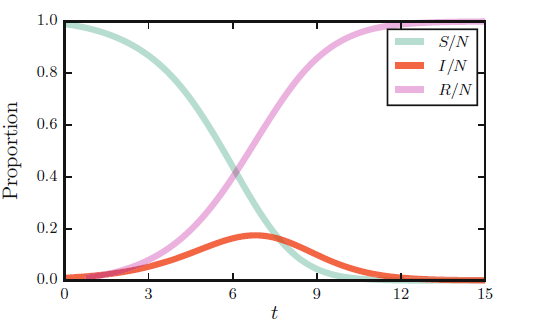
\includegraphics[scale=.8, keepaspectratio]{sir_model}
			\caption{dipendenza temporale delle dimensioni relative dei compartimenti rispetto alla totalità della popolazione; $ \gamma = 1 $ e $ \beta = 1.6 $. \cite{Kiss}}
			\label{fig:evolution}
		\end{center}
	\end{figure}

che mette in luce la relazione fra il numero di riproduzione di base e la dimensione finale dell'epidemia, $\left[ N - S_\infty \right ] $.\footnote{Qui abbiamo sottinteso di star cercando delle soluzioni costanti della coppia di equazioni differenziali, $ \left( S_\infty, I_\infty \right ) $; partendo dal presupposto che, a $ t = 0 $, $ S_0 + I_0 = N $ e ricordando che $ lim_{t\to \infty} I(t) = I_\infty = 0 $, risulta che $ \lim_{t\to \infty} S(t) + I(t) = S_\infty $.}